\chapter{Vektorielle Geometrie}


\section{Vektoren}
    \begin{Definition}
        Ein Vektor ist Element eines Vektorraums.
    \end{Definition}\\
    \paragraph{} Vektorräume, wir erinnern uns zurück. Verknüpfungen, inverse Elemente und die dazugehörenden Gesetze, konsequente Definitionen und mathematische Korrektheit, die guten alten Zeiten...\\
    Tatsächlich kann ein Vektor in den meisten Fällen als Verschiebung bezeichnet werden, \textbf{nicht aber als Pfeil oder Strich!}\\

    \subsection{Besondere Vektoren}

        \subsubsection{Der Ortsvektor}

            \paragraph{} Der Vektor von $O$ auf den Punkt $P$, geschrieben als $\vv{OP}$ oder $\vv{o}$.\\
            \paragraph{} Hat $P$ die Koordinaten $(P_1|P_2|...|P_n)$, so besitzt $\vv{o}$ die Darstellung $\left(\begin{array}{c} P_1 \\ P_2 \\ ...\\P_n\end{array}\right)$.

        \subsubsection{Der Nullvektor}

            \paragraph{} Der Vektor mit Wert $\left(\begin{array}{c} 0 \\ 0 \\ ...\\0\end{array}\right)$, er hat keine und alle Richtungen zugleich.
            \begin{Bemerkung}
                Er ist somit das neutrale Element der Vektoraddition.
            \end{Bemerkung}

        \subsubsection{Der Verbindungsvektor}

            \paragraph{} Der Vektor $\vv{AB}$ ist der Vektor, der den Punkt $A$ auf den Punkt $B$ abbildet. Er ist definiert als:\\ $\vv{AB}=\vv{OB}-\vv{OA}$, woraus folgt, dass: \begin{center} $\vv{AB} = \left(\begin{array}{c} b_1 - a_1 \\ b_2 - a_2 \\ ... \\ b_n - a_n \end{array}\right)$. \end{center}

        \subsubsection{Der Gegenvektor}

            \paragraph{} Der Gegenvektor zu $\vv{AB}$ ist $\vv{BA}$, definiert als  $-\vv{AB}$.
            \begin{Bemerkung}
                Er ist somit das inverse Element der Vektoraddition.
            \end{Bemerkung}

    \subsubsection{Der Einheitsvektor}

        \subsubsubsection{Norm eines Vektors}

            \paragraph{} Die Norm eines Vektors ist anschaulich als seine Länge zu interpretieren. Der Betrag, wie sie ebenfalls genannt wird, eines Vektors $\vv{v}$ ist folgendermaßen definiert: $\text{|}\vv{v}\text{|} = \sqrt{\displaystyle\sum_{i=1}^{n}v_{i^2}} ; \vv{v}\in\R^n$.
            \\
            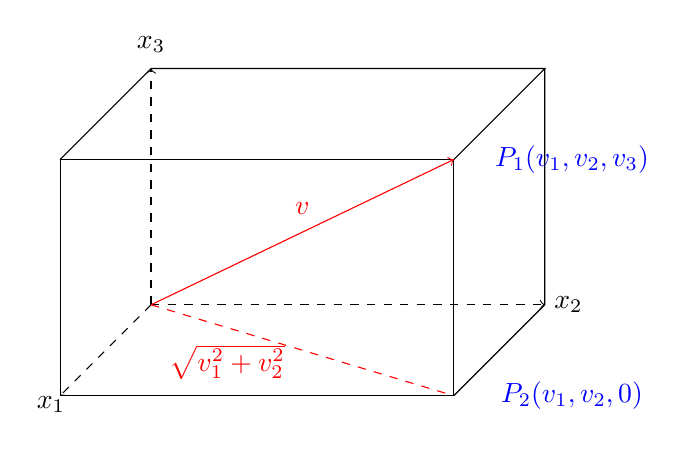
\begin{tikzpicture}
                \draw[dashed, ->] (0,0,0) -- (0,0,3);
                \draw[dashed, ->] (0,0,0) -- (5,0,0);
                \draw[dashed, ->] (0,0,0) -- (0,3,0);
                \draw[dashed, color=red] (0,0,0) -- (5,0,3);
                \draw (0,0,3) -- (5,0,3) -- (5,3,3) -- (0,3,3) -- (0,0,3);
                \draw (0,3,3) -- (0,3,0) -- (5,3,0) -- (5,3,3);
                \draw (5,3,0) -- (5,0,0) -- (5,0,3);
                \draw[->, color=red] (0,0,0) -- (5,3,3);
                \draw (0,0,3.3) node {$x_1$};
                \draw (5.3,0,0) node {$x_2$};
                \draw (0,3.3,0) node {$x_3$};
                \draw (2.5,1.8,1.5) node [color=red]{$\vv{v}$};
                \draw (6.5,3,3) node [color=blue]{$P_1 (v_1, v_2, v_3)$};
                \draw (6.5,0,3) node [color=blue]{$P_2 (v_1, v_2, 0)$};
                \draw (1.7,0,1.9) node [color=red]{$\sqrt{v_1^{2}+v_2^{2}}$};
            \end{tikzpicture}
            \paragraph{} Anhand dieser Graphik lässt sich die Berechnung der Norm eines Vektors $\vv{v}\in\R^3$ verdeutlichen. Für diesen glit: $\text{|}\vv{v}\text{|}=\sqrt{v_1^{2}+v_2^{2}+v_3^{2}}$.
            \paragraph{} Ein Vektor, dessen Norm 1 beträgt wird als normiert oder Einheitsvektor bezeichnet. Für jeden Vektor $\vv{v}\in\R^{3}$ existiert ein Einheitsvektor $\vv{v^{*}}$ , der folgendermaßen definiert wird: $\vv{v^{*}}=\frac{1}{\text{|}\vv{v}\text{|}}*\vv{v}$.

\section{Linearkombination}

    \paragraph{} Vektoren lassen sich allgemein mit der additiven Verknüpfung des Vektorraumes verknüpfen. Diese Verknüpfung zwischen zwei beliebigen Vektoren $\vv{v}$ und $\vv{u}$ erfolgt, wie auch schon im Teil Verbindungsvektor gezeigt wird, wie folgt: $\vv{v}+\vv{u}=\left(\begin{array}{c}{v_1+u_1 \\ v_2+u_2 \\ ... \\ v_n+u_n}\end{array}\right)$.
    \\
    \begin{Definition}
       Eine Familie von Vektoren $\vv{a_1},\vv{a_2},...,\vv{a_n}\in V$ wird als linear abhängig bezeichnet, wenn die Gleichung: \\$r_1\cdot\vv{a_1}+r_2\cdot\vv{a_2}+...+r_n\cdot\vv{a_n}=\vv{0};r_i\in\R$ nicht nur die triviale Lösung $r_1=r_2=...=r_n=0$ besitzt. Existiert nur diese Lösung, ist die Familie linear unabhägig.
    \end{Definition}
    \paragraph{} Anders gesagt, ist eine Familie von Vektoren linear abhängig, wenn sich einzelne Vektoren dieser Familie als Linearkombination von einer beliebigen Anzahl anderer Vektoren der Familie darstellen lassen.
    \begin{Bemerkung}
      Eine linear abhängige Familie \textbf{aus genau zwei} Vektoren wird als kollinear bezeichnet.
      \\
      Eine linear abhängige Familie \textbf{aus genau drei} Vektoren, als komplanar.
    \end{Bemerkung}
\section{Basen und Erzeugendensystem}
    \paragraph{} Eine endliche Anzahl von Vektoren $\vv{a_1},\vv{a_2},...,\vv{a_n}\in V$ heißt Erzeugendensystem, wenn sich \texbf{jeder} Vektor $\vv{v}\in V$ als Linearkombination dieser Vektoren schreiben lässt. Um ein Erzeugendensystem zu bilden benötigt man mindestens die Anzahl Vektoren, die der Anzahl von Dimensionen von $\vv{v}$ entspricht. Wenn man \textbf{genau} diese Anzahl besitzt, spricht man von einer Basis.
    \subsection{Besondere Basen}
        \subsubsection{Orthogonalbasis}
        \paragraph{} Sind die Vektoren der Basis paarweise orthogonal zueinander, so spricht man von einer \textbf{Orthogonalbasis}.
        \subsubsection{Orthonormalbasis}
        \paragraph{} Sind die Vektoren zusätzlich zu dieser Bedingung normiert, wird sie als \textbf{Orthonormalbasis} bezeichnet. Die einfachste und meist benutzte Basis des $\R^3$ besteht aus den drei Vektoren $\vv{e_1}=\left(\begin{array}{c}{1\\0\\0}\end{array}\right),\vv{e_2}=\left(\begin{array}{c}{0\\1\\0}\end{array}\right),\vv{e_3}=\left(\begin{array}{c}{0\\0\\1}\end{array}\right)$. Sie wird als \textbf{Standardbasis} des $\R^3$ bezeichnet. Vektoren wie $\vv{v}=\left(\begin{array}{c}{2\\3\\8}\end{array}\right)$ lassen sich als eine Linearkombination der drei Vektoren der Standardbasis darstellen: $\vv{v}=2\cdot\vv{e_1}+3\cdot\vv{e_2}+8\cdot\vv{e_3}$.
    \subsection{Basistransformation}

        \paragraph{} Bilden die Vektoren $\vv{a_1},\vv{a_2},...,\vv{a_n}$ eine Basis des $n$-dimensionalen Vektorraums $V$ und sei der Vektor $\vv{v}=\left(\begin{array}{c}{v_1\\v_2\\...\\v_n}\end{array}\right);\vv{v}\in V$. Dann gilt wie üblich: $\vv{v}=v_1\cdot\vv{a_1}+v_2\cdot\vv{a_2}+...+v_n\cdot\vv{a_n}$. Sei eine weitere Basis $\vv{b_1},\vv{b_2},...,\vv{b_n}$ des selben Vektorraumes, so besitzt der Vektor $\vv{v}$ andere Koordinaten: $\vv{v}=\left(\begin{array}{c}{v'_1\\v'_2\\...\\v'_n}\end{array}\right)$. Dabei muss gelten: $\vv{v}=v_1\cdot\vv{a_1}+v_2\cdot\vv{a_2}+...+v_n\cdot\vv{a_n}=v'_1\cdot\vv{b_1}+v'_2\cdot\vv{b_2}+...+v'_n\cdot\vv{b_n}$.

        \begin{Bemerkung}
            Um die Koordinaten eines Vektors in einer anderen Basis als der Aktuellen zu bestimmen, löst man diese Gleichung, die sich ergibt.
        \end{Bemerkung}

        \begin{Beispiel}
            Basis 1: Standardbasis des $\R^3$, Basis 2: $\vv{b_1}=\left(\begin{array}{c}{4\\9\\-1}\end{array}\right), \vv{b_2}=\left(\begin{array}{c}{-2\\-2\\8}\end{array}\right), \vv{b_3}=\left(\begin{array}{c}{1\\3\\1}\end{array}\right)$, Vektor $\vv{v}=\left(\begin{array}{c}{-5\\3\\2}\end{array}\right)$ (in der Standardbasis des $\R^3$)
            \\
            $\vv{v}=-5\cdot\vv{a_1}+3\cdot\vv{a_2}+2\cdot\vv{a_3}=r\cdot\vv{b_1}+s\cdot\vv{b_2}+t\cdot\vv{b_3}$
            $\Leftrightarrow \begin{vmatrix}4r & -2s & t & = & -5 \\
                                            9r & -2s & 3t & = & 3 \\
                                            -r & 8s & t & = & 2
                            \end{vmatrix}
             \\
             \\
             \Leftrightarrow \begin{vmatrix}-r & 8s & t & = & 2 \\
                                            0 & 30s & 5t & = & 3 \\
                                            0 & 70s & 12t & = & 21
                             \end{vmatrix}
             \\
             \\
             \Leftrightarrow \begin{vmatrix}-r & 8s & t & = & 2 \\
                                            0 & 30s & 5t & = & 3 \\
                                            0 & 0 & \frac{1}{3}\cdot t & = & 14
                             \end{vmatrix}
             \\
             \\
             \Leftrightarrow \begin{vmatrix}t & = & 99.2 \\
                                            s & = & -6.9 \\
                                            r & = & 42
                             \end{vmatrix}
            \\
            \\
            \mathbb{L}=\{ 42,|6.9|99.2 \}$
            \\
            Daraus lässt sich folgern: $\vv{v}=42\cdot\vv{b_1}-6.9\cdot\vv{b_2}+99.2\cdot\vv{b_3}=\left(\begin{array}{c}{42\\-6.9\\99.2}\end{array}\right)$ (in der anderen Basis).
            \\
            Ich hab keinen Plan, ob meine Berechnungen stimmen, aber es ging vorerst um das Prinzip. Könnte jemand mal bitte nachrechnen?

        \end{Beispiel}


\section{Winkel zwischen Vektoren}\subsection{Orientierte Winkel}

\section{Geraden}
\section{Ebenen}
\section{Skalarprodukt}
